%%%%%%%%%%%%%%%%%%%%%%%%%%%%%%%%%%%%%%%%%
% Beamer Presentation
% LaTeX Template
% Version 1.0 (10/11/12)
%
% This template has been downloaded from:
% http://www.LaTeXTemplates.com
%
% License:
% CC BY-NC-SA 3.0 (http://creativecommons.org/licenses/by-nc-sa/3.0/)
%
%%%%%%%%%%%%%%%%%%%%%%%%%%%%%%%%%%%%%%%%%

%----------------------------------------------------------------------------------------
%	PACKAGES AND THEMES
%----------------------------------------------------------------------------------------

\documentclass{beamer}

\usepackage[polish, english]{babel}
\usepackage[T1]{fontenc}
\usepackage[utf8]{inputenc}


\mode<presentation> {

% The Beamer class comes with a number of default slide themes
% which change the colors and layouts of slides. Below this is a list
% of all the themes, uncomment each in turn to see what they look like.

%\usetheme{default}
%\usetheme{AnnArbor}
%\usetheme{Antibes}
%\usetheme{Bergen}
%\usetheme{Berkeley}
%\usetheme{Berlin}
%\usetheme{Boadilla}
%\usetheme{CambridgeUS}
%\usetheme{Copenhagen}
%\usetheme{Darmstadt}
%\usetheme{Dresden}
%\usetheme{Frankfurt}
%\usetheme{Goettingen}
%\usetheme{Hannover}
%\usetheme{Ilmenau}
%\usetheme{JuanLesPins}
%\usetheme{Luebeck}
%\usetheme{Madrid}
%\usetheme{Malmoe}
%\usetheme{Marburg}
%\usetheme{Montpellier}
%\usetheme{PaloAlto}
%\usetheme{Pittsburgh}
%\usetheme{Rochester}
%\usetheme{Singapore}
%\usetheme{Szeged}
\usetheme{Warsaw}

% As well as themes, the Beamer class has a number of color themes
% for any slide theme. Uncomment each of these in turn to see how it
% changes the colors of your current slide theme.

%\usecolortheme{albatross}
%\usecolortheme{beaver}
%\usecolortheme{beetle}
%\usecolortheme{crane}
%\usecolortheme{dolphin}
%\usecolortheme{dove}
%\usecolortheme{fly}
%\usecolortheme{lily}
%\usecolortheme{orchid}
%\usecolortheme{rose}
%\usecolortheme{seagull}
%\usecolortheme{seahorse}
%\usecolortheme{whale}
%\usecolortheme{wolverine}

%\setbeamertemplate{footline} % To remove the footer line in all slides uncomment this line
%\setbeamertemplate{footline}[page number] % To replace the footer line in all slides with a simple slide count uncomment this line

%\setbeamertemplate{navigation symbols}{} % To remove the navigation symbols from the bottom of all slides uncomment this line
}

\usepackage{graphicx} % Allows including images
\usepackage{booktabs} % Allows the use of \toprule, \midrule and \bottomrule in tables

\AtBeginSection[]{
  \begin{frame}
  \vfill
  \centering
  \begin{beamercolorbox}[sep=8pt,center,shadow=true,rounded=true]{title}
    \usebeamerfont{title}\secname\par%
  \end{beamercolorbox}
  \vfill
  \end{frame}
}

\newenvironment{VerbExample}
{\example\semiverbatim}
{\endsemiverbatim\endexample}

%----------------------------------------------------------------------------------------
%	TITLE PAGE
%----------------------------------------------------------------------------------------

\title[GADT]{Statically type checked DSLs with GADTs} % The short title appears at the bottom of every slide, the full title is only on the title page

\author{Konrad Werbliński} % Your name
\institute[UWr] % Your institution as it will appear on the bottom of every slide, may be shorthand to save space

\date{\today} % Date, can be changed to a custom date

\begin{document}

\begin{frame}
\titlepage % Print the title page as the first slide
\end{frame}

\section{ADT}

\begin{frame}[fragile]
  \frametitle{ADT}
  In their simplest form they are similar to enum in C++
  \begin{VerbExample}
data OS = Windows | Linux | MacOS

enum class OS \{Windows, Linux, MacOS\};
  \end{VerbExample}
\end{frame}


\begin{frame}[fragile]
  \frametitle{ADT}
  \begin{VerbExample}
isGoodSystem os = case os of
  Windows -> False
  Linux -> True
  MacOS -> True

-------------------------------
isGoodSystem Windows = False
isGoodSystem Linux = True
isGoodSystem MacOS = True
  \end{VerbExample}
\end{frame}


\begin{frame}[fragile]
  \frametitle{ADT}
  But each constructor can holds values! So they are similar to combination
  of variant and tuple, but each element of the alternative is named.
  \begin{VerbExample}

data Shape
  = Circle Float Color
  | Rectangle Float Float Color

  \end{VerbExample}
\end{frame}

\begin{frame}[fragile]
  \frametitle{ADT}
  They can also be generic.
  \begin{VerbExample}
data Optional a = Nothing | Just a

Just 5 :: Optional Int
Just "Konrad" :: Optional String
Nothing :: Optional a
  \end{VerbExample}
\end{frame}

\begin{frame}[fragile]
  \frametitle{ADT}
  They can also be recursive.
  \begin{VerbExample}
data List a = Empty | Cons a (List a)

-- In Haskell:

data [a] = [] | a : [a]

Usage:
5 : [1, 3, 4] = [5, 1, 3, 4]

head :: [a] -> a
head (x : _) = xs
  \end{VerbExample}
\end{frame}


\begin{frame}[fragile]
  \frametitle{ADT}
  They can also be recursive.
  \begin{VerbExample}
data Tree a = Leaf | Node (Tree a) a (Tree a)

t :: Tree Int
t = Node Leaf 44 (Node Leaf 42 Leaf)

44
 \\
  42
\end{VerbExample}
\end{frame}

\begin{frame}[fragile]
  \frametitle{ADT}
  Let's look at the simple expressions DSL
  \begin{VerbExample}
data Expr
  = ENum Int
  | EStr String
  | EPlus Expr Expr
  | ECat Expr Expr
  | ELen Expr

EPlus (ENum 44) (ELen (EStr "Munich"))
\end{VerbExample}
\end{frame}

\begin{frame}[fragile]
  \frametitle{ADT}
  Let's try to evaluate expressions.
  \begin{VerbExample}
data Value = VInt Int | VStr String

eval :: Expr -> Value
eval (EInt n) = VInt
...
eva1 (EPlus e1 e2) =
  let (VInt n1) = eval e1 in
  let (VInt n2) = eval e2 in
  VInt (n1 + n2)
...

But this will crash for:
EPlus (EStr "Munich") (EInt 44)
\end{VerbExample}
\end{frame}

\begin{frame}[fragile]
  \frametitle{ADT}
  \begin{itemize}
    \item We would like to make our DLS type safe!
    \item But how to do it?
    \item We can define expressions as Expr a, and use the type
    parameter to carry necessary information!
  \end{itemize}
\end{frame}

\begin{frame}[fragile]
  \frametitle{ADT}
  \begin{VerbExample}
data Expr a
  = ENum Int
  | EStr String
  | EPlus (Expr Int) (Expr Int)
  | ECat (Expr String) (Expr String)
  | ELen (Expr String)
\end{VerbExample}

However, above code would not work, we are not setting the type parameter
of the created types.

\end{frame}

\begin{frame}[fragile]
  \frametitle{ADT}
We can wrapper functions over constructors, to set the type parameter.
  \begin{VerbExample}
eNum :: Int -> Expr Int
eNum n = ENum n

ePlus :: Expr Int -> Expr Int -> Expr Int
ePlus e1 e2 = EPlus e1 e2

eLen :: Expr String -> Expr Int
eLen e = ELen e
\end{VerbExample}

\end{frame}

\begin{frame}[fragile]
  \frametitle{ADT}
However, we can do better! :D
\end{frame}

\section{GADT}

\begin{frame}[fragile]
  \frametitle{GADT}
We can use GADTs!
  \begin{VerbExample}
data Expr a where
  ENum :: Int -> Expr Int
  EStr :: String -> Expr String
  EPlus :: Expr Int -> Expr Int -> Expr Int
  ECat :: Expr String -> Expr String -> Expr String
  ELen :: Expr String -> Expr Int
\end{VerbExample}
\end{frame}

\begin{frame}[fragile]
  \frametitle{GADT}
Now the following code will produce type error!
  \begin{VerbExample}
EPlus (EStr "Munich") (EInt 44)
\end{VerbExample}
\end{frame}

\begin{frame}[fragile]
  \frametitle{GADT}
Eval function also becomes nicer!
  \begin{VerbExample}
eval :: Expr a -> a
eval (EInt n) = n
...
eva1 (EPlus e1 e2) =
  let n1 = eval e1 in
  let n2 = eval e2 in
  n1 + n2
...
\end{VerbExample}
\end{frame}


\begin{frame}[fragile]
  \frametitle{GADT - More complex DSL}
Statically type checked printf
  \begin{VerbExample}
data Format t where
  Str :: Format a -> Format (String -> a)
  Inr :: Format a -> Format (Int -> a)
  Flt :: Format a -> Format (Float -> a)
  Lit :: String -> Format a -> Format a
  Eol :: Format a -> Format a
  End :: Format ()

Lit "Hello" (Str (Lit "! Answer:" (Inr End)))
:: Format (String -> Int -> ())
\end{VerbExample}
\end{frame}

\begin{frame}[fragile]
  \frametitle{GADT - More complex DSL}
Statically type checked String formatting
  \begin{VerbExample}
printf :: Format a -> a
printf End = ()
printf (Lit s format) = putStr s `seq` printf format
printf (Eol format) = putStrLn "" `seq` printf format
printf (Str format) =
  \\x -> putStr x `seq` printf format
printf (Inr format) =
  \\x -> (putStr . intToString) x `seq` printf formats
printf (Flt format) =
  \\x -> (putStr . floatToString) x `seq` printf format
  \end{VerbExample}
\end{frame}

\begin{frame}[fragile]
  \frametitle{GADT - More complex DSL}
Thus:
  \begin{VerbExample}
Lit "Hello" (Str (Lit "! Answer:" (Inr End)))
:: Format (String -> Int -> ())

printf (Lit "Hello" (Str (Lit "! Answer:" (Inr End))))
:: String -> Int -> ()

printf
(Lit "Hello" . Str . Lit "! Answer:" . Inr \$ End)
"Konrad" 42
  \end{VerbExample}
\end{frame}


\begin{frame}[fragile]
  \frametitle{GADT - empty types as labels}

Let's imagine a tree that holds different types of data
in the left and right sons.
  \begin{VerbExample}
data Tree
  = Leaf
  | LeftSon Int Tree Tree
  | RightSon String Tree Tree

But nothing prevents us from creating:
Left (Left 42 Leaf Leaf) (Left 44 Leaf Leaf)

  \end{VerbExample}
\end{frame}

\begin{frame}[fragile]
  \frametitle{GADT - empty types as labels}
How to make sure that the construction of a tree is correct.
We can use GADTs!, and empty types for labeling.
  \begin{VerbExample}
data Left
data Right

data Tree side where
  Leaf :: Tree a
  LeftSon ::
    Int -> Tree Left -> Tree Right -> Tree Left
  RightSon ::
    String -> Tree Left -> Tree Right -> Tree Right
  \end{VerbExample}
\end{frame}


\begin{frame}[fragile]
  \frametitle{GADT - encoding natural numbers as empty types}
  \begin{VerbExample}
data Zero
data Succ n

type One = Succ Zero
type Two = Succ One
//type Two = Succ (Succ Zero)
...

To make life easier we will write
0, 1, 2, 3 ... instead of types
Zero, One, Two, Three, ...
  \end{VerbExample}
\end{frame}


\begin{frame}[fragile]
  \frametitle{GADT - Vec}
  \begin{VerbExample}
data Vec n a where
  [] :: Vec 0 a
  (:) :: a -> Vec n a -> Vec (Succ n) a
  \end{VerbExample}
\end{frame}

\begin{frame}[fragile]
  \frametitle{GADT - Vec}
  \begin{VerbExample}
[42, 5, 44, 59] :: Vec 4 Int

["Haskell", "OCaml", "Bestrafer"] :: Vec 3 String

[] :: Vec 0 a
  \end{VerbExample}
\end{frame}

\begin{frame}[fragile]
  \frametitle{GADT - Vec}
  \begin{VerbExample}
map :: (t1 -> t2) -> Vec n t1 -> Vec n t2
map _ [] = []
map f (head : tail) = f head : map f tail
  \end{VerbExample}
\end{frame}

\begin{frame}[fragile]
  \frametitle{GADT - Vec}
  \begin{VerbExample}
map f [1, 2, 3, 4] = [f 1, f 2, f 3, f 4]
  \end{VerbExample}
\end{frame}

\begin{frame}[fragile]
  \frametitle{GADT - Vec}
  \begin{VerbExample}
map fac [1, 2, 3, 4] = [1, 2, 6, 24]
  \end{VerbExample}
\end{frame}

\begin{frame}[fragile]
  \frametitle{GADT - Vec}
  \begin{VerbExample}
map :: (t1 -> t2) -> Vec n t1 -> Vec n t2
map _ [] = []
map f (head : tail) = f head : map f tail
  \end{VerbExample}
\end{frame}

\begin{frame}[fragile]
  \frametitle{GADT - Vec}
  \begin{VerbExample}
map :: (t1 -> t2) -> List t1 -> List t2
map _ _ = []
  \end{VerbExample}
\end{frame}

\begin{frame}[fragile]
  \frametitle{GADT - Vec}
  \begin{VerbExample}
map :: (t1 -> t2) -> List t1 -> List t2
map f list = [f (head list)]
  \end{VerbExample}
\end{frame}

\begin{frame}[fragile]
  \frametitle{GADT - Vec}
  \begin{VerbExample}
map :: (t1 -> t2) -> Vec n t1 -> Vec n t2
map _ [] = []
map f (head : tail) = f head : map f tail
  \end{VerbExample}
\end{frame}

\begin{frame}[fragile]
  \frametitle{GADT - matrix operations}
    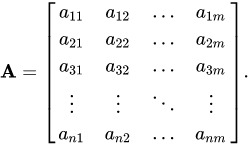
\includegraphics[scale=0.5]{matrix.png}
    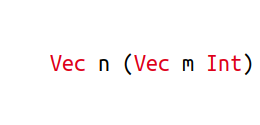
\includegraphics[scale=0.5]{vec.png}
\end{frame}

\begin{frame}[fragile]
  \frametitle{GADT - matrix operations}
    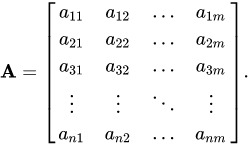
\includegraphics[scale=0.5]{matrix.png}
    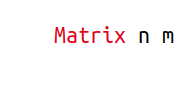
\includegraphics[scale=0.5]{mat.png}
\end{frame}

\begin{frame}[fragile]
  \frametitle{GADT - matrix operations}
  \begin{VerbExample}
transpose :: Matrix n m -> Matrix m n
transpose matrix =
  let indices = range (len (head matrix)) in
  map (\\i -> column i matrix) indices
  \end{VerbExample}
\end{frame}

\begin{frame}[fragile]
  \frametitle{GADT - matrix operations}
  \begin{VerbExample}
mult :: Matrix n m -> Matrix m k -> Matrix n k
mult a b = map (\\v -> multVec v b) a
  \end{VerbExample}
\end{frame}

\begin{frame}[fragile]
  \frametitle{GADT - matrix operations}
  \begin{VerbExample}
multVec :: Vec n Int -> Matrix n m -> Vec m Int
  \end{VerbExample}
\end{frame}

\begin{frame}[fragile]
  \frametitle{GADT - matrix operations}
  \begin{VerbExample}
mult :: Matrix n m -> Matrix m k -> Matrix n k
mult a b = map (\\v -> multVec v b) a
  \end{VerbExample}
\end{frame}

\begin{frame}[fragile]
  \frametitle{GADT - red black tree}
  \begin{VerbExample}
data Black
data Red

data RBTree col blackHeight t where
  Black :: RBTree c1 n t ->
           t ->
           RBTree c2 n t ->
           RBTree Black (S n) t
  Red :: RBTree Black n t ->
         t ->
         RBTree Black n t ->
         RBTree Red n t
  Empty :: RBTree Black 0 t
  \end{VerbExample}
\end{frame}

\end{document}